\documentclass[twoside]{article}
\setlength{\oddsidemargin}{0 in}
\setlength{\evensidemargin}{0 in}
\setlength{\topmargin}{-0.6 in}
\setlength{\textwidth}{6.5 in}
\setlength{\textheight}{8.5 in}
\setlength{\headsep}{0.75 in}
\setlength{\parindent}{0 in}
\setlength{\parskip}{0.1 in}

\usepackage{url}
\usepackage{titlesec}
\setcounter{secnumdepth}{3}
\usepackage{palatino}
\usepackage{marginnote}
\usepackage{multirow}
\usepackage{easybmat,bigdelim,arydshln}
\usepackage[authoryear,round]{natbib}
\usepackage{amssymb,amsmath,amsthm,amsfonts}
\usepackage{mathtools}
\usepackage{caption}
\usepackage{hyperref}
\usepackage{tcolorbox}
\tcbuselibrary{skins, breakable, theorems}
\usepackage{newpxtext,newpxmath}
\usepackage{longtable}
\usepackage{enumitem}
\makeatletter

\let\bar\overline

\setlist[itemize]{topsep=0pt,leftmargin=10pt,itemsep=-0.2em}
\usepackage{xcolor}
\usepackage{tikz}
\usepackage{pgfplots}
\pgfplotsset{compat = newest}
\usetikzlibrary{patterns,decorations.pathreplacing,decorations.markings,fit,shapes.geometric,angles,quotes,arrows}
\usepgfplotslibrary{fillbetween}

\usepackage{ifthen}
\usepackage{tikz-3dplot}

\pgfdeclarelayer{ft}
\pgfdeclarelayer{bg}
\pgfsetlayers{bg,main,ft}

\hypersetup{
    colorlinks,
    citecolor=red,
    filecolor=black,
    linkcolor=violet,
    urlcolor=blue
}

\definecolor{myblue}{cmyk}{1,.72,0,.38}
\definecolor{mypurple}{cmyk}{.57,1,0,.58}
\definecolor{myred}{cmyk}{0,.88,.88,.58}
\definecolor{mygreen}{cmyk}{1,0,.69,.66}
\definecolor{myorange}{cmyk}{0,.58,100,.20}
\definecolor{glaucous}{rgb}{0.38, 0.51, 0.71}

\makeatletter
\renewcommand{\thefigure}{\thesection.\arabic{figure}}
\newtheoremstyle{indented}
  {3pt}% space before
  {3pt}% space after
  {\addtolength{\@totalleftmargin}{3.5em}
   \addtolength{\linewidth}{-3.5em}
   \parshape 1 3.5em \linewidth}% body font
  {}% indent
  {\bfseries}% header font
  {.}% punctuation
  {.5em}% after theorem header
  {}% header specification (empty for default)
\makeatother

\newcommand{\ind}{\perp\!\!\!\perp}

\theoremstyle{definition}
\newtheorem{defin}{Definition}[section] % Creates a new counter, number within section
\newtheorem{prt}[defin]{Remark} 
\newtheorem{prts}[defin]{Remarks} % Again share defin's counter
\newtheorem{exmp}[defin]{Example} % etc.
\newtheorem*{note}{Note}
\tcbuselibrary{theorems}

% use counter*=defin to make each tcbtheorem share defin's counter

\newtcbtheorem[use counter*=defin, number within=section]{definition}{Definition}{enhanced, breakable,
    colback = white, colframe = red!55!black, colbacktitle = red!55!black, attach boxed title to top left = {yshift = -2.5mm, xshift = 3mm}, boxed title style = {sharp corners},fonttitle=\bfseries}{def}

\newtcbtheorem[use counter*=defin, number within=section]{theorem}{Theorem}{enhanced, breakable,
    colback = white, colframe = blue!45!black, colbacktitle = blue!45!black, attach boxed title to top left = {yshift = -2.5mm, xshift = 3mm}, boxed title style = {sharp corners},fonttitle=\bfseries}{thm}
    
\newtcbtheorem[use counter*=defin, number within=section]{proposition}{Proposition}{enhanced, breakable,
    colback = white, colframe = teal, colbacktitle = teal, attach boxed title to top left = {yshift = -2.5mm, xshift = 3mm}, boxed title style = {sharp corners},fonttitle=\bfseries}{prop}

\newtcbtheorem[use counter*=defin, number within=section]{lemma}{Lemma}{enhanced, breakable,
    colback = white, colframe = orange!80!black, colbacktitle = orange!80!black, attach boxed title to top left = {yshift = -2.5mm, xshift = 3mm}, boxed title style = {sharp corners},fonttitle=\bfseries}{lemma}

\newtcbtheorem[use counter*=defin, number within=section]{corollary}{Corollary}{enhanced, breakable,
    colback = white, colframe = yellow!60!black, colbacktitle = yellow!60!black, attach boxed title to top left = {yshift = -2.5mm, xshift = 3mm}, boxed title style = {sharp corners},fonttitle=\bfseries}{corol}

\newtcbtheorem[use counter*=defin, number within=section]{algorithm}{Algorithm}{enhanced, breakable,
    colback = white, colframe = green!55!black, colbacktitle = green!55!black, attach boxed title to top left = {yshift = -2.5mm, xshift = 3mm}, boxed title style = {sharp corners},fonttitle=\bfseries}{algm}
%\newtcolorbox{example}[1]{enhanced, breakable, colback = white, colframe = orange!85!black, colbacktitle = orange!85!black, attach boxed title to top left = {yshift = -2.5mm, xshift = 3mm}, boxed title style = {sharp corners},fonttitle=\bfseries, title={Example: #1}}

\newtcbox{\myhl}[1][white]
  {on line, arc = 0pt, outer arc = 0pt,
    colback = #1!20!white, colframe = #1!50!black,
    boxsep = 0pt, left = 1pt, right = 1pt, top = 1pt, bottom = 1pt, boxrule = 0pt, bottomrule =0pt, toprule =0pt}
    
\newtcbox{\myhlrule}[1][white]
  {on line, arc = 0pt, outer arc = 0pt,
    colback = #1!20!white, colframe = #1!50!black,
    boxsep = 0pt, left = 1pt, right = 1pt, top = 1pt, bottom = 1pt, boxrule = 0pt, bottomrule =0.5pt, toprule =0.5pt}
%
% The following commands set up the lecnum (lecture number)
% counter and make various numbering schemes work relative
% to the lecture number.
%

\renewcommand{\thepage}{\arabic{page}}
\renewcommand{\thesection}{\arabic{section}}
\renewcommand{\theequation}{\arabic{equation}}
\renewcommand{\thefigure}{\arabic{figure}}
\renewcommand{\thetable}{\arabic{table}}

\newcommand{\sidenotes}[1]{\marginnote{\raggedright\scriptsize#1}}
%
% The following macro is used to generate the header.
%
\newcommand{\lecture}[5]{
   \pagestyle{myheadings}
   \thispagestyle{plain}
   \newpage
   \setcounter{page}{1}
   \noindent
   \begin{center}
   \framebox{
      \vbox{\vspace{2mm}
    \hbox to 6.28in { {\bf 
	\hfill \today} }
       \vspace{4mm}
       \hbox to 6.28in { {\Large \hfill Note: #1  \hfill} }
       \vspace{2mm}
       \hbox to 6.28in { {\it #2 \hfill by #3} }
      \vspace{2mm}}
   }
   \end{center}
   %\markboth{Week #1: #2}{Week #1: #2}

   {\bf Key points}: {#4}

   {\bf Disclaimer}: {\it #5}
   \vspace*{4mm}
}
%

\tikzset{-stealth-/.style={decoration={
  markings,
  mark=at position #1 with {\arrow{stealth}}},postaction={decorate}}}

  \tikzset{tangent/.style={
    decoration={
        markings,% switch on markings
        mark=
            at position #1
            with
            {
                \coordinate (tangent point-\pgfkeysvalueof{/pgf/decoration/mark info/sequence number}) at (0pt,0pt);
                \coordinate (tangent unit vector-\pgfkeysvalueof{/pgf/decoration/mark info/sequence number}) at (1,0pt);
                \coordinate (tangent orthogonal unit vector-\pgfkeysvalueof{/pgf/decoration/mark info/sequence number}) at (0pt,1);
            }
    },
    postaction=decorate
},
use tangent/.style={
    shift=(tangent point-#1),
    x=(tangent unit vector-#1),
    y=(tangent orthogonal unit vector-#1)
},
use tangent/.default=1}

\tikzstyle{terminator} = [rectangle, draw, thick, text centered, rounded corners, minimum height=2em]
\tikzstyle{process} = [rectangle, draw, thick, text centered, minimum height=2em]
\tikzstyle{decision} = [diamond, draw, thick, text centered, minimum width=3cm, minimum height=0.5cm]
\tikzstyle{data}=[trapezium, draw, thick, text centered, trapezium left angle=60, trapezium right angle=120, minimum height=2em]
\tikzstyle{arrow} = [thick,->,>=stealth]

\begin{document}
\lecture{Contamination Bias in Linear Regressions}{as in \citet{goldsmith2022contamination}}{Sai Zhang}{The contamination bias arises in multiple-treatment regression even when the treatment assignment is as good as random, due to the \textbf{inherent nonlinear dependence} of mutually exclusive treatment indicators.}{This note is built on \citet{goldsmith2022contamination}.}

\section{Motivation}
Consider the regression
\begin{equation}\label{eq:linear_binarytreat}
    Y_i = \alpha + \beta D_i + \gamma W_i + U_i
\end{equation}
where
\begin{itemize}
    \item $D_i\in\left\{ 0,1 \right\}$ is a single treatment indicator
    \item $W_i\in\left\{ 0,1 \right\}$ is a single binary control
    \item $U_i$ is a mean-zero residual uncorrelated with $D_i$ and $W_i$
\end{itemize}
Assume the (within-strata) treatment assignment is random, i.e., conditionally independent of potential outcomes given the control:
\begin{equation}\label{eq:conditional_indep}
    \left( Y_i(0),Y_i(1) \right) \bot D_i \mid W_i
\end{equation}
where $Y_i(d)$ is the outcome of individual $i$ when $D_i=d$, $i$'s treatment effect is given by $\tau_i = Y_i(1)-Y_i(0)$, and the realized outcome is $Y_i=Y_i(0)+\tau_i D_i$.

By \citet*{angrist1998estimating}, $\beta$ in Eq (\ref{eq:linear_binarytreat}) identifies a weighted average of within-strata ATEs with \myhl[myblue]{\textbf{convex}} weights:
\begin{align}\label{eq:angrist_weightedATE}
    \beta &= \phi \tau(0) + (1-\phi) \tau(1) &\text{where }\phi &= \frac{\mathrm{var}(D_i\mid W_i=0)\Pr (W_i=0)}{\sum_{w=0}^1 \mathrm{var}(D_i\mid W_i=w)\Pr (W_i=w)}\in[0,1]
\end{align}
and 
$$
\tau(w) = \mathbb{E}\left[ Y_i(1) - Y_i(0) \mid W_i=w\right]
$$
is the ATE in the strata indexed by control $W_i = w$.

By appying the Frisch-Waugh-Lovell (FWL) Theorem, $\beta$ can be written as the univariate regression coefficient of regression $Y_i$ on $\tilde{D}_i$\footnote{$\tilde{D}_i$ is the residual of regressing $D_i$ on $W_i$ and a constant: $$D_i = a + b W_i + \tilde{D}_i$$}:
\begin{align}
    \beta = \frac{\mathbb{E}\left[\tilde{D}_iY_i\right]}{\mathbb{E}\left[\tilde{D}^2_i\right]} &= \frac{\mathbb{E}\left[\tilde{D}_iY_i(0)\right]}{\mathbb{E}\left[\tilde{D}^2_i\right]} + \frac{\mathbb{E}\left[\tilde{D}_iD_i\tau_i\right]}{\mathbb{E}\left[\tilde{D}^2_i\right]} \nonumber \\ 
    &=\frac{\mathbb{E}\left[\mathbb{E}\left[\tilde{D}_iY_i(0)\mid W_i\right]\right]}{\mathbb{E}\left[\tilde{D}^2_i\right]} + \frac{\mathbb{E}\left[\mathbb{E}\left[\tilde{D}_iD_i\tau_i\mid W_i\right]\right]}{\mathbb{E}\left[\tilde{D}^2_i\right]} \nonumber \\
    &= \frac{\mathbb{E}\left[\mathbb{E}\left[\tilde{D}_i\mid W_i\right]\mathbb{E}\left[Y_i(0)\mid W_i\right]\right]}{\mathbb{E}\left[\tilde{D}^2_i\right]} + \frac{\mathbb{E}\left[ \mathbb{E}\left[\tilde{D}_iD_i\mid W_i\right] \mathbb{E}\left[\tau_i\mid W_i\right] \right]}{\mathbb{E}\left[\tilde{D}^2_i\right]} \label{eq:keystep_meanindep}\\
    & = 0 + \frac{\mathbb{E}\left[ \mathrm{var}(D_i\mid W_i)\tau(W_i) \right]}{\mathbb{E}\left[ \mathrm{var}(D_i\mid W_i) \right]} \nonumber
\end{align}

for the derivation in Eq. (\ref{eq:keystep_meanindep}) to work, the key underlying point is that $\mathbb{E}\left[\tilde{D}_i\mid W_i\right]=0$, i.e., $\tilde{D}_i$ is \textcolor{myblue}{\textbf{mean-independent}} of $W_i$ and the propensity score $\mathbb{E}\left[ D_i\mid W_i \right]$ is \textcolor{myblue}{\textbf{linear}} since $W_i$ is \textcolor{myred}{\textbf{binary}}. 

\paragraph*{Where contamination bias arises} Now add an \textbf{additional treatment arm}: consider 2 \myhl[myblue]{\textbf{mutually exclusive}} interventions: $D_i \in \left\{0,1,2\right\}$, represented by a vector of 2 treatment indicators $\mathbf{X}_i = \left(X_{i1},X_{i2}\right)'$ where 
\begin{align*}
    X_{i1}&=\mathbf{1}\left\{D_i=1\right\} & X_{i2}&=\mathbf{1}\left\{D_i=2\right\}
\end{align*}
this yields the regression 
\begin{equation}\label{eq:example_2treatment}
    Y_i = \alpha + \beta_1 X_{i1} + \beta_2 X_{i2} + \gamma W_i + U_i
\end{equation}
now the observe outcome is given by $Y_i = Y_i(0) +\tau_{i1}X_{i1}+ \tau_{i2}X_{i2}$
\begin{align*}
    \tau_{i1} &= Y_i(1)- Y_i(0) & \tau_{i2} &= Y_i(2)-Y_i(0)
\end{align*}
hence, some heterogeneity in treatment effect emerges. Still, assume $\mathbf{X}_i$ is conditionally independent of $Y_i(d)$ given control $W_i$
$$
\left( Y_i(0),Y_i(1),Y_i(2) \right) \bot \mathbf{X}_i \mid W_i
$$
If we still use FWL theorem to derive $\beta_1$
\begin{equation}\label{eq:FWL_2treat_coef}
    \beta_1 = \frac{\mathbb{E}\left[ \tilde{X}_{i1}Y_i \right]}{\mathbb{E}\left[ \tilde{X}^2_{i1} \right]} = \frac{\mathbb{E}\left[ \tilde{X}_{i1}Y_i(0) \right]}{\mathbb{E}\left[ \tilde{X}^2_{i1} \right]} + \frac{\mathbb{E}\left[ \tilde{X}_{i1} X_{i1}\tau_{i1} \right]}{\mathbb{E}\left[ \tilde{X}^2_{i1} \right]} + \frac{\mathbb{E}\left[ \tilde{X}_{i1} X_{i2}\tau_{i2} \right]}{\mathbb{E}\left[ \tilde{X}^2_{i1} \right]}
\end{equation}
where $\tilde{X}_{i1}$ is obtained by running $X_{i1} = a+bX_{i2}+cW_i +\tilde{X}_{i1}$. Now, the issues is that $X_{i1}$ and $X_{i2}$ are \textbf{mutually exclusive}:
\begin{itemize}
    \item If $X_{i2} = 1$: $X_{i1}=0$, \myhl[myred]{\textbf{not}} depends on $W_i$
    \item If $X_{i2} = 0$: the mean of $X_{i1}$ depends on $W_i$
\end{itemize}
hence in general
$$
\tilde{X}_{i1} \neq X_{i1} - \mathbb{E}\left[ X_{i1}\mid W_i,X_{i2} \right]
$$
which means that we can only derive $\beta_1$ from Eq. (\ref{eq:FWL_2treat_coef}) as 
\begin{align}
    \beta_1 &= \frac{\mathbb{E}\left[ \tilde{X}_{i1}Y_i(0) \right]}{\mathbb{E}\left[ \tilde{X}^2_{i1} \right]} + \frac{\mathbb{E}\left[ \tilde{X}_{i1} X_{i1}\tau_{i1} \right]}{\mathbb{E}\left[ \tilde{X}^2_{i1} \right]} + \frac{\mathbb{E}\left[ \tilde{X}_{i1} X_{i2}\tau_{i2} \right]}{\mathbb{E}\left[ \tilde{X}^2_{i1} \right]} \nonumber \\
    &= 0 + \mathbb{E}\left[\lambda_{11}(W_i)\tau_1 (W_i)\right] + \mathbb{E}\left[ \lambda_{12}(W_i)\tau_2(W_i) \right]
\end{align}
breakdown each term:
\begin{itemize}
    \item $\mathbb{E}\left[\tilde{X}_{i1}Y_i(0)\right]/\mathbb{E}\left[\tilde{X}_{i1}^2\right]$: FWL regression residuals are \textbf{uncorrelated} with $Y_i(0)$
    \begin{align*}
       X_{i1}&=a + bX_{i2} + cW_i +\tilde{X}_{i1} \\
        \textcolor{myred}{\xRightarrow[\text{\tiny on both sides}]{\text{\tiny purge $W_i$}}} \tilde{\tilde{X}}_{i1} &= \mu_1\tilde{\tilde{X}}_{i2} + \tilde{X}_{i1} \Rightarrow \tilde{X}_{i1} = \tilde{\tilde{X}}_{i1} - \mu_1 \tilde{\tilde{X}}_{i2} \xRightarrow{\left( Y_i(0),Y_i(1),Y_i(2) \right) \bot \mathbf{X}_i \mid W_i} \mathbb{E}\left[\tilde{X}_{i1}Y_i(0)\right] = 0
    \end{align*}
    \item $\mathbb{E}\left[ \tilde{X}_{i1} X_{i1}\tau_{i1} \right]/\mathbb{E}\left[ \tilde{X}^2_{i1} \right]$: similarly to Eq. (\ref{eq:keystep_meanindep}), 
    \begin{align*}
        \frac{\mathbb{E}\left[ \tilde{X}_{i1} X_{i1}\tau_{i1} \right]}{\mathbb{E}\left[ \tilde{X}^2_{i1} \right]} &= \frac{\mathbb{E}\left[ \mathbb{E}\left[\tilde{X}_{i1} X_{i1}\tau_{i1}\mid W_i\right] \right]}{\mathbb{E}\left[ \tilde{X}^2_{i1} \right]} \textcolor{myred}{\xRightarrow{\left( Y_i(0),Y_i(1),Y_i(2) \right) \bot \mathbf{X}_i \mid W_i}} = \mathbb{E}\left[ \underbrace{\frac{\mathbb{E}\left[\tilde{X}_{i1}X_{i1}\mid W_i\right]}{\mathbb{E}\left[\tilde{X}_{i1}^2\right]}}_{\equiv \lambda_{11}(W_i)}\tau_1(W_i) \right]
    \end{align*}
    here, $\lambda_{11}(W_i)$ is still non-negative and average to one, hence similar to Eq. (\ref{eq:keystep_meanindep}), this term is still a convex average of the conditional ATEs $\tau_1(W_i)$.
    \item $\mathbb{E}\left[ \tilde{X}_{i1} X_{i2}\tau_{i2} \right]/\mathbb{E}\left[ \tilde{X}^2_{i1} \right]$: on the contrary,
    \begin{align*}
        \frac{\mathbb{E}\left[ \tilde{X}_{i1} X_{i2}\tau_{i2} \right]}{\mathbb{E}\left[ \tilde{X}^2_{i1} \right]} &= \frac{\mathbb{E}\left[ \mathbb{E}\left[\tilde{X}_{i1} X_{i2}\tau_{i2}\mid W_i\right] \right]}{\mathbb{E}\left[ \tilde{X}^2_{i1} \right]} \textcolor{myred}{\xRightarrow{\left( Y_i(0),Y_i(1),Y_i(2) \right) \bot \mathbf{X}_i \mid W_i}} = \mathbb{E}\left[ \underbrace{\frac{\mathbb{E}\left[\tilde{X}_{i1}X_{i2}\mid W_i\right]}{\mathbb{E}\left[\tilde{X}_{i1}^2\right]}}_{\equiv \lambda_{12}(W_i)} \tau_2(W_i)\right]
    \end{align*}
    here $X_{i2} \neq X_{i1} - \mathbb{E}\left[ X_{i1} \mid W_i, X_{i2} \right] $, hence $\lambda_{12}(W_i)$ is generally \myhl[myred]{\textbf{non-zero}}. This term is essentially the \textbf{contamination bias}.
\end{itemize}

\paragraph*{How to simply understand contamination bias?}
As shown above,
\begin{equation*}
    \mathbb{E}\left[ \frac{\mathbb{E}\left[\tilde{X}_{i1}X_{i2}\mid W_i\right]}{\mathbb{E}\left[\tilde{X}_{i1}^2\right]} \tau_2(W_i)\right] \equiv \mathbb{E}\left[ \lambda_{12}(W_i) \tau_2(W_i)\right] \neq 0
\end{equation*}
arises because $\tilde{X}_{i1}$ is \textbf{uncorrelated} with $X_{i2}$ by construction, but \textbf{NOT} conditionally independent of $X_{i2}$. To understand this, consider a two-step residualization:
\begin{itemize}
    \item \underline{\textbf{Step 1}}: first, demean $X_{i1}$ and $X_{i2}$, conditional on $W_i$
    \begin{align*}
        \hat{X}_{i1} &= X_{i1} - \mathbb{E}\left[X_{i1} \mid W_i\right] = X_{i1}- p_1(W_i) & \hat{X}_{i2}&= X_{i2}-\mathbb{E}\left[X_{i2}\mid W_i\right] = X_{i2} - p_2(W_i)
    \end{align*}
    where $p_j(W_i) = \mathbb{E}\left[X_{ij}\mid W_i\right]$ gives the propensity score for treatment $j$
    \item \underline{\textbf{Step 2}}: run a bivarite regression 
    $$
    \hat{X}_{i1} = \alpha \hat{X}_{i2} + \tilde{X}_{i1}
    $$
\end{itemize}
Therefore, when the propensity scores vary across different strata ($W_i=w_a$ v.s. $W_i=w_b$), that is $$ p_j(w_a) \neq p_j(w_b) $$
the regression in Step 2 would also preserve this strata heterogeneity, leading to the \textit{contamination weight} $\lambda_{12}(W_i)$ non-zero.

\paragraph*{A numerical example}
Consider $W_i \in \left\{0,1\right\}$ and a two-arm treatment assignment $D_i\in\left\{ 0,1,2 \right\}$
\begin{table}[ht]
    \begin{center}
      \begin{tabular}{l|ccc}
        & $D_i=0$ & $D_i=1$ & $D_i=2$ \\ \hline
        $W_i=0$ & 50\% & 5\% & 45\% \\
        $W_i=1$ & 10\% & 45\% & 45\%
        \end{tabular}
    \end{center}
\end{table}

and the 2 strata have equal number of observations, then we have the propensity score
\begin{align*}
    p_1(0)&=0.05 & p_2(0)&=0.45 & p_1(1)&=p_2(1)=0.45
\end{align*}
Then the \textit{contamination weights} are
\begin{align*}
    \lambda_{12}(W_i=0) &= \frac{\mathbb{E}\left[\tilde{X}_{i1}X_{i2}\mid W_i=0\right]}{\mathbb{E}\left[\tilde{X}^2_{i1}\right]} = \frac{99}{106} & \lambda_{12}(W_i=1) &= \frac{\mathbb{E}\left[\tilde{X}_{i1}X_{i2}\mid W_i=1\right]}{\mathbb{E}\left[\tilde{X}^2_{i1}\right]} = -\frac{99}{106}
\end{align*}
If we calculate the conditional correlation of the 2 within-strata residualzied treatments
\begin{equation*}
    \mathrm{corr}\left(\tilde{X}_{i1},\tilde{X}_{i2}\mid W_i\right) = -\sqrt{\frac{p_1(W_i)}{1-p_1(W_i)}} \cdot \sqrt{\frac{p_2(W_i)}{1-p_2(W_i)}}
\end{equation*}
then we have 
\begin{align*}
    \mathrm{corr}\left( \tilde{X}_{i1},\tilde{X}_{i2} \mid W_i=0 \right) &= -0.2075 & \mathrm{corr}\left( \tilde{X}_{i1},\tilde{X}_{i2} \mid W_i=1 \right)&=-0.8182
\end{align*}
the overall regression of $\tilde{X}_{i1}$ on $\tilde{X}_{i2}$ would be correlated with $X_{i2}$ within each strata, hence misspecified (see Figure \ref{fig:misspecify_example} for an illustration).
\begin{figure}[ht]
    \centering
    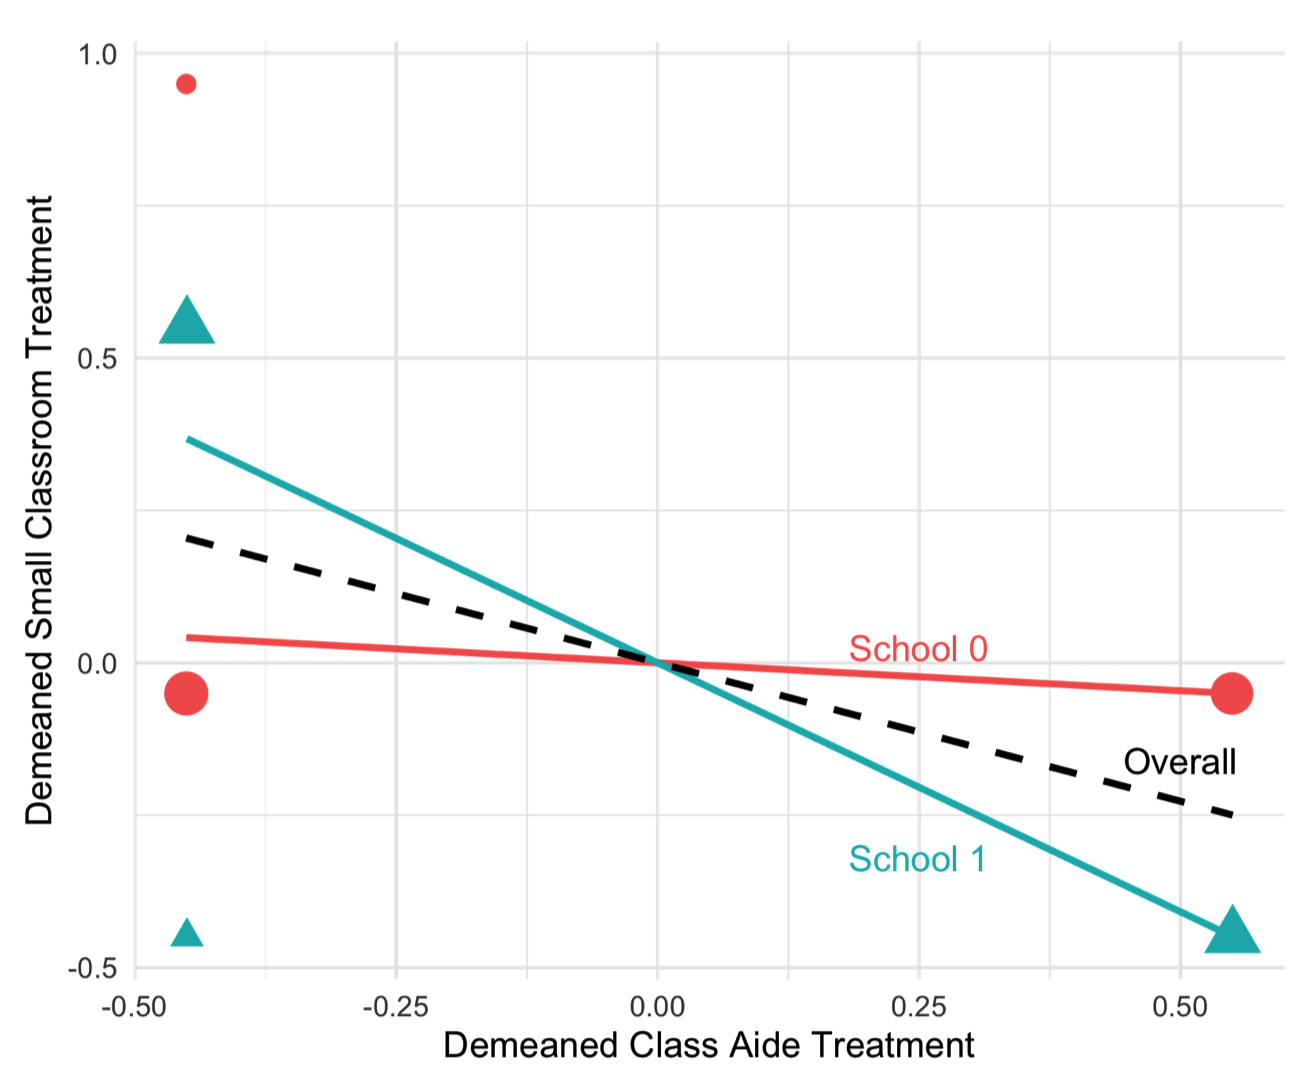
\includegraphics[width = 0.6 \textwidth]{figures/example_misspecify.png}
    \caption{An Example of Contamination Bias \citep[Figure 1]{goldsmith2022contamination}}\label{fig:misspecify_example}
\end{figure}

\paragraph*{When is the contamination bias $0$?} 
We have derived
$$
\beta_1 = \mathbb{E}\left[\lambda_{11}(W_i)\tau_1(W_i)\right] + \underbrace{\mathbb{E}\left[\lambda_{12}(W_i)\tau_2(W_i)\right]}_{\textcolor{myred}{\text{contamination bias}}}
$$
now consider 2 scenarios where the contamination bias vanishes
\begin{itemize}
    \item \textbf{\underline{Case 1}}: constant treatment effects of the 2nd treatment arm $\tau_2(W_i)\equiv \tau_2$, then 
    \begin{equation*}
        \beta_1 = \mathbb{E}\left[\lambda_{11}(W_i)\tau_1(W_i)\right] + \mathbb{E}\left[\lambda_{12}(W_i)\tau_2(W_i)\right] = \mathbb{E}\left[\lambda_{11}(W_i)\tau_1(W_i)\right] + \underbrace{\mathbb{E}\left[\lambda_{12}(W_i)\right]}_{=0}\tau_2 = \mathbb{E}\left[\lambda_{11}(W_i)\tau_1(W_i)\right]
    \end{equation*}
    more generally, the \myhl[myblue]{\textbf{less heterogeneous}} the treatment effect of the 2nd treatment arm $\tau_2(W_i)$ is (or the \myhl[myblue]{\textbf{less correlated}} it is with $\lambda_{11}(W_i)$), the smaller the contamination bias is.
    \item \textbf{\underline{Case 2}}: $X_{i1}$ and $X_{i2}$ are \myhl[myblue]{\textbf{independent}} conditional on $W_i$\footnote{That is, they are no longer mutually exclusive: individuals can be assigned to both treatment arms with a non-zero probability.}, that is 
    $$ \mathbb{E}\left[X_{i1}\mid W_i, X_{i2}\right] = \mathbb{E}\left[X_{i1}\mid W_i\right]$$
    which solves the issue naturally, guaranteeing 
    $$
    \tilde{X}_{i1} = X_{i1} - \mathbb{E}\left[X_{i1}\mid W_i,X_{i2}\right] = X_{i1} - \mathbb{E}\left[X_{i1}\mid W_i\right]
    $$
    naturally, conditional independence of $X_{i1}$ and $X_{i2}$ brings contamination bias to 0, reducing it to a single treatment problem.
\end{itemize}

\paragraph*{How to solve the issue?} 
An intuitive and simple solution to the problem is just including an interaction term between $W_i$ and $X_{i2}$ in Eq. (\ref{eq:example_2treatment})
\begin{equation*}
    Y_i = \alpha + \beta_1 X_{i1} + \beta_2 X_{i2} + \gamma W_i + \xi\textcolor{myred}{ X_{i2}\times W_i} +V_i
\end{equation*}
then the FWL regression 
$$
X_{i1} = a + bX_{i2} + cW_i + d\textcolor{myred}{X_{i2}\times X_i} + \tilde{X}_{i1}
$$
is saturated and capture the nonlinearity in $\mathbb{E}\left[ X_{i1}\mid W_i,X_{i2} \right]$.

\section{General Characterization}
Now, consider a general characterization of the intuition above. For a partially linear model
\begin{equation}\label{eq:partial_linear_model}
    Y_i = \mathbf{X}'_i\boldsymbol{\beta} + g(\mathbf{W}_i) + U_i
\end{equation}
where 
\begin{itemize}
    \item treatment indictors $\mathbf{X}_i = \left( X_{i1},\cdots,X_{iK} \right)' $: $X_{ik} = \mathbf{1}\left\{D_i = k\right\}$ for a $K-$arm mutually exclusive treatment assignment $D_k\in \left\{0,\cdots, K\right\}$
    \item vector of control variables $\mathbf{W}_i$ 
\end{itemize}
and $\boldsymbol{\beta}$ and $g$ are defined as
\begin{equation}\label{eq:minimization_problem}
    (\boldsymbol{\beta},g) = \arg\min_{\tilde{\boldsymbol{\beta}}\in \mathbb{R}^K,\tilde{g}\in \mathcal{G}} \mathbb{E}\left[ \left( Y_i - \mathbf{X}'_i\tilde{\boldsymbol{\beta}}-\tilde{g}(\mathbf{W}_i) \right)^2 \right]
\end{equation}
this characterization includes 2 of the most common applications
\begin{itemize}
    \item \myhl[myblue]{\textbf{multi-arimed RCT}}: $\mathbf{W}_i$ is the vector of indicators for experimental strata, within which $\mathbf{X}_i$ is randomly assigned to individual $i$, $g$ is linear
    \item \myhl[myblue]{\textbf{two-way FEs}}: For a fixed unit $j\in\left\{1,\cdots,J\right\}$ and period $t\in\left\{ 1,\cdots,T \right\}$, $W_i = (J_i,T_i)$ indicates the underlying unit and period for each observation $i$ in a panel data where $J_i=j,T_i=t$, and $g(W_i) = \alpha + \left(\mathbf{1}\left\{J_i=2\right\},\cdots,\mathbf{1}\left\{J_i=n\right\},\mathbf{1}\left\{T_i=2\right\},\mathbf{1}\left\{T_i=T\right\}\right)'\boldsymbol{\gamma}$ includes unit and period indicators. $\mathbf{X}_i$ contains \textbf{lead} and \textbf{lag} indicators relative to a treatment adoption date $A(j)\in \left\{ 1,\cdots, T \right\}$
\end{itemize}

\subsection{Derive Treatment Coefficients} 
To derive $\mathbf{\beta}$, solve the minimization problem in Eq. (\ref{eq:minimization_problem}), get
\begin{equation}\label{eq:beta_vector_derived}
    \boldsymbol{\beta} = \mathbb{E}\left[ \tilde{\mathbf{X}}_i \tilde{\mathbf{X}}_i' \right]^{-1}\mathbf{E}[\tilde{\mathbf{X}}_i Y_i]
\end{equation}
where $\tilde{\mathbf{X}}_i$ is the residual vector from projecting $\mathbf{X}_i$ onto the controls:
$$
\tilde{\mathbf{X}}_{ik} = \mathbf{X}_{ik} - \arg\min_{\tilde{g}\in\mathcal{G}}\mathbb{E}\left[\left(\tilde{\mathbf{X}}_{ik}-\tilde{g}\left({\mathbf{W}}_i\right)\right)^2\right]
$$
Following FWL theorem, each treatment coefficient of $\boldsymbol{\beta}$ can be written as 
$$
\boldsymbol{\beta}_k = \frac{\mathbb{E}\left[\tilde{\tilde{\mathbf{X}}}_{ik}Y_i\right]}{\mathbb{E}\left[\tilde{\tilde{\mathbf{X}}}^2_{ik}\right]}
$$
where $\tilde{\tilde{\mathbf{X}}}_{ik}$ is the residual from regression $\tilde{\mathbf{X}}_{ik}$ on $\tilde{\mathbf{X}}_{i,-k} = \left(\tilde{\mathbf{X}}_{i1},\cdots, \tilde{\mathbf{X}}_{i,k-1},\tilde{\mathbf{X}}_{i,k+1},\cdots,\tilde{\mathbf{X}}_{iK}\right)'$.

\subsection{Causal interpretation}
Let $Y_i(k)$ denote the potential outcome of unit $i$ when $D_i=k$, then observed outcomes are given by 
$$
Y_i = Y_i(D_i) = Y_i(0) + \mathbf{X}_i'\tau_i
$$
where $\tau_i$ is the vector of treatment effects, $\tau_{ik} = Y_i(k)-Y_i(0)$. 
\begin{itemize}
    \item \myhl[myblue]{\textbf{conditional ATE}}: The conditional expectation of the vector of treatment effects given by the controls is 
    $$
    \boldsymbol{\tau}(\mathbf{W}_i) = \mathbb{E}\left[\tau_i\mid \mathbf{W_i}\right]
    $$
    and $\tau_k(\mathbf{W}_i)$ is the {\textbf{conditional ATE}} of the $k$th treatment.
    \item \myhl[myblue]{\textbf{propensity scores}}: let $$\mathbf{p}(\mathbf{W}_i) = \mathbb{E}\left[ \mathbf{X}_i\mid\mathbf{W_i} \right]$$ denote the vector of propensity scores, with components being $\mathbf{p}_k(\mathbf{W}_i) = \Pr \left(D_i=k\mid \mathbf{W}_i\right)$
\end{itemize}

\paragraph*{2 assumptions}
\begin{itemize}
    \item[\textbf{A1}]\label{assumption1} \myhl[myred]{\textbf{mean-independence}} of the potential outcomes and treatment, conditional on the controls:
    $$
    \mathbb{E}\left[Y_i(k)\mid D_i, \mathbf{W}_i\right] = \mathbb{E}\left[ Y_i(k) \mid \mathbf{W}_i \right],\forall k
    $$
    a \textit{sufficient} condition for this assumption is the conditional independence of treatment and potential outcomes (e.g., random assignment)
    \begin{equation*}
        \left(Y_i(0),\cdots,Y_i(K)\right) \bot D_i\mid \mathbf{W}_i
    \end{equation*}
    \item[\textbf{A2}]\label{assumption2} \myhl[myred]{\textbf{propensity scores}} must be captured by the covariate adjustment function family $\mathcal{G}$:
    \begin{align}
        \mathbf{p}_k\left( w \right) &= \mathbb{E}\left[\mathbf{X}_{ik}\mid \mathbf{W}_i = w\right] \in \mathcal{G},\forall k \label{eq:assumption2_1}\\
        \mu_0\left( w \right) &= \mathbb{E}\left[Y_i(0)\mid \mathbf{W}_i = w\right] \in \mathcal{G}\label{eq:assumption2_2}
    \end{align}
    one of Eq. (\ref{eq:assumption2_1}) and Eq. (\ref{eq:assumption2_2}) must be satisfied, then OVB can be avoided.
\end{itemize}

\paragraph*{Two simple cases}
Under 2 scenarios, there would be no bias 
\begin{itemize}
    \item \myhl[myblue]{\textbf{homogeneous} (constant within treatment arm $k$) \textbf{treatment effect}}:
    Consider $\tau_{ik}=\tau_k$ for all $k$, then $$Y_i = Y_i(0)+ \mathbf{X}_i'\boldsymbol{\tau}$$ where $\boldsymbol{\tau} = \left(\tau_1,\cdots,\tau_k\right)'$, the coefficient vector identifies $\boldsymbol{\tau}$ is 
    \begin{align*}
        \boldsymbol{\beta} = \mathbb{E}\left[\tilde{\mathbf{X}}_i\tilde{\mathbf{X}}_i'\right]^{-1}\mathbb{E}\left[\tilde{\mathbf{X}}_iY_i\right] &= \mathbb{E}\left[\tilde{\mathbf{X}}_i\tilde{\mathbf{X}}_i'\right]^{-1}\left(\mathbb{E}\left[\tilde{\mathbf{X}}_iY_i(0)\right] + \mathbb{E}\left[\tilde{\mathbf{X}}_i{\mathbf{X}}_i'\right]\boldsymbol{\tau}\right)\\
        &= \mathbb{E}\left[\tilde{\mathbf{X}}_i\tilde{\mathbf{X}}_i'\right]^{-1}\left(\mathbb{E}\left[\tilde{\mathbf{X}}_iY_i(0)\right] + \mathbb{E}\left[\tilde{\mathbf{X}}_i\tilde{\mathbf{X}}_i'\right]\boldsymbol{\tau}\right)\\
        &= \mathbb{E}\left[\tilde{\mathbf{X}}_i\tilde{\mathbf{X}}_i'\right]^{-1} \mathbb{E}\left[\tilde{\mathbf{X}}_iY_i(0)\right] + \boldsymbol{\tau} = \mathbb{E}\left[\tilde{\mathbf{X}}_i\tilde{\mathbf{X}}_i'\right]^{-1} \mathbb{E}\left[\tilde{\mathbf{X}}_iY_i(0)\right] + \boldsymbol{\tau}
    \end{align*}
    by the Law of Iterated Expectations, $\mathbb{E}\left[\tilde{\mathbf{X}}Y_i(0)\right] = \mathbb{E}\left[\tilde{\mathbf{X}}_i \mathbb{E}\left[Y_i(0)\mid \mathbf{W}_i\right]\right] = \mathbb{E}\left[\mathbb{E}\left[\tilde{\mathbf{X}}_i\mid \mathbf{W}_i\right] \mathbb{E}\left[Y_i(0)\mid \mathbf{W}_i\right]\right]$, then 
    \begin{itemize}
        \item under Eq. (\ref{eq:assumption2_1}), $\mathbb{E}\left[\tilde{\mathbf{X}}_i \mid \mathbf{W}_i\right] = 0$
        \item under Eq. (\ref{eq:assumption2_2}), $\mathbb{E}\left[\tilde{\mathbf{X}}_i \mathbb{E}\left[Y_i(0)\mid \mathbf{W}_i\right] \right] = \mathbb{E}\left[ \tilde{\mathbf{X}}_i\mu_0(\mathbf{W}_i) \right] =0$
    \end{itemize}
    no omitted variable bias.
    \item \myhl[myblue]{\textbf{heterogeneous} treatment effects, \textbf{single} treatment arm}: the coefficient is 
    \begin{align*}
        \boldsymbol{\beta} = \mathbb{E}\left[ \tilde{\mathbf{X}}_i \tilde{\mathbf{X}}_i' \right]^{-1}\mathbf{E}[\tilde{\mathbf{X}}_i Y_i] =\frac{\mathbb{E}\left[\tilde{\mathbf{X}}_i {\mathbf{X}}_i \tau_i\right]}{\mathbb{E}\left[\tilde{\mathbf{X}}_i^2\right]} = \mathbb{E}\left[ \frac{\mathbb{E}\left[\tilde{\mathbf{X}}_i {\mathbf{X}}_i \mid \mathbf{W}_i\right]}{\mathbb{E}\left[\tilde{\mathbf{X}}_i{\mathbf{X}}_i\right]} \cdot \tau(\mathbf{W}_i)\right]
    \end{align*}
    $\boldsymbol{\beta}$ is just a weighted average of heterogeneous treatment effects with weight $\lambda_{11}(\mathbf{W}_i) = \frac{\mathbb{E}\left[\tilde{\mathbf{X}}_i {\mathbf{X}}_i \mid \mathbf{W}_i\right]}{\mathbb{E}\left[\tilde{\mathbf{X}}_i{\mathbf{X}}_i\right]}$. And, 
    \begin{itemize}
        \item under Eq. (\ref{eq:assumption2_1}), $\mathbb{E}\left[\tilde{\mathbf{X}}_i\mathbf{X}_i\mid \mathbf{W}_i\right] = \mathbb{E}\left[\tilde{\mathbf{X}}_i^2\mid \mathbf{W}_i\right] = \mathrm{Var}\left(\mathbf{X}_i\mid \mathbf{W}_i\right)$, the weight is \textbf{\underline{non-negative}}
        \item under Eq. (\ref{eq:assumption2_2}) but \textit{not} Eq. (\ref{eq:assumption2_1}), negative weights could arise.
    \end{itemize}
\end{itemize}

\paragraph*{Contamination bias}
In the general model (\ref{eq:partial_linear_model}), contamination bias arises

\begin{proposition}{Contamination Bias in the Partial Linear Model (\ref{eq:partial_linear_model})}{contamination_bias}
    Under Assumption \hyperref[assumption1]{1} and \hyperref[assumption1]{2}, the treatment coefficients in the partial linear model (\ref{eq:partial_linear_model}) identify 
    \begin{equation}
        \boldsymbol{\beta}_k = \mathbb{E}\left[ \lambda_{kk}(\mathbf{W}_i)\tau_k(\mathbf{W}_i) \right] + \textcolor{myred}{\sum_{l\neq k}\mathbb{E}\left[\lambda_{kl}(\mathbf{W}_i)\tau_l(\mathbf{W}_i)\right] }
    \end{equation}
    where the weights
    \begin{align*}
        \lambda_{kk}(\mathbf{W}_i) &= \frac{\mathbb{E}\left[\tilde{\tilde{\mathbf{X}}}_{ik}\mathbf{X}_{ik}\mid \mathbf{W}_k\right]}{\mathbf{E}\left[\tilde{\tilde{\mathbf{X}}}^2_{ik}\right]} & \lambda_{kl}(\mathbf{W}_i) &= \frac{\mathbb{E}\left[\tilde{\tilde{\mathbf{X}}}_{ik}\mathbf{X}_{il}\mid \mathbf{W}_k\right]}{\mathbf{E}\left[\tilde{\tilde{\mathbf{X}}}^2_{ik}\right]}
    \end{align*}
    satisfy that 
    \begin{align*}
        \mathbb{E}\left[\lambda_{kk}(\mathbf{W}_i)\right] &= 1 & \mathbb{E}\left[\lambda_{kl}(\mathbf{W}_i)\right] & =0
    \end{align*}
    and under Eq (\ref{eq:assumption2_1}), $\lambda_{kk}(\mathbf{W}_i)\geq 0, \forall k$.
\end{proposition}

here, the coefficient is decomposed into 2 terms:
\begin{itemize}
    \item a weighted average of conditional ATEs: $\mathbb{E}\left[ \lambda_{kk}(\mathbf{W}_i)\tau_k(\mathbf{W}_i) \right]$
    \begin{itemize}
        \item It generalizes the coefficient in the single treatment case
        \item The weights $\lambda_{kk}\left(\mathbf{W}_i\right)$ average to 1, and convex under Eq. (\ref{eq:assumption2_1})
    \end{itemize}
    
    \item \myhl[myred]{\textbf{Contamination bias}}: a weighted average of treatment effects of \textit{other} treatments $\tau_l(\mathbf{W}_i)$
\end{itemize}

\paragraph*{When there is no contamination bias}
The contamination bias persists generally, with several exceptions:
\begin{itemize}
    \item $\lambda_{kl}(\mathbf{W}_i) = \mathbb{E}\left[\tilde{\tilde{\mathbf{X}}}_{ik}\mathbf{X}_{il}\mid \mathbf{W}_k\right]/\mathbf{E}\left[\tilde{\tilde{\mathbf{X}}}^2_{ik}\right] = 0$ almost surely, $\forall l\neq k$. Consider 
    $$
    \mathbb{E}\left[ \tilde{\tilde{\mathbf{X}}}_{ik} \mid \mathbf{X}_{i,-k},\mathbf{W}_i \right] = 0
    $$
    or equivalently,
    $$
    \mathbb{E}\left[ \tilde{\tilde{\mathbf{X}}}_{ik} \mid \mathbf{X}_{i,-k},\mathbf{W}_i \right] = \mathbf{X}'_{i,-k}\boldsymbol{\alpha} +g_k(\mathbf{W}_i)
    $$
    However, when the treatment arms are mutually exclusive, that is, $\mathbf{X}_{ik}=0$ if the unit is assigned to one of the other treatments regardless of $\mathbf{W}_i$, hence it's always true that 
    $$
    {\alpha}_l = -g_k(\mathbf{W}_i)
    $$
    for all elements $\alpha_l$ of $\boldsymbol{\alpha}$, implying that the assignment of treatment does not depend on $\mathbf{W}_i$, which is generally not ture unless the \underline{propensity score $p_k(\mathbf{W}_i)$ is \textbf{constant}}.
    \item the conditional effects of the other treatments are \textbf{homogeneous} s.t. $\tau_l(\mathbf{W}_i) = \tau_l$
    \item the weights $\lambda_{kl}(\mathbf{W}_i)$ and conditional ATEs $\tau_l(\mathbf{W}_i)$ are \textbf{\underline{uncorrelated}} with each other
    \begin{itemize}
        \item more generally, contamination bias is less concerning when $\lambda_{kl}(\mathbf{W}_i)$ and $\tau_l(\mathbf{W}_i)$ are weakly correlated: that is, the factors influencing treatment effect heterogeneity are largely \textbf{\underline{unrelated}} to the factors influencing the treatment assignment process.
    \end{itemize}
\end{itemize}

\paragraph*{Some remarks} on the general characterization of contamination bias 
\begin{itemize}
    \item[R1] in the multiple treatment case, contamination bias generally arises regardless of Assumption \hyperref[assumption2]{2}, when one use an \myhl[myred]{\textbf{additive}} covariate adjustment, even the covariate specifications are flexible.
    \item[R2] the contamination bias can be \myhl[myred]{\textbf{bounded}} by the identified contamination weights $\lambda_{kl}(\mathbf{W}_i)$ and the heterogeneity in conditional ATEs $\tau_l(\mathbf{W}_i)$
    \item[R3] \myhl[myred]{\textbf{negative weighting}}: when the treatments are \textbf{\textit{not}} mutually exclusive, $\lambda_{kk}(\mathbf{W}_i)$ may still be negative under Eq. (\ref{eq:assumption2_1}).
    
    \underline{\textit{Note}}: for the two-way FE regressions, none of the recent alternative specifications for $g$\footnote{For example, linear trends, interacted FEs, or other extensions of the basic parallel trends model.} are flexible enough to capture the degenerate propensity scores, hence Eq. (\ref{eq:assumption2_1}) in general won't hold.
    \item[R4] \myhl[myred]{\textbf{IV}}: following Prop.\ref{prop:contamination_bias}, 
    \begin{itemize}
        \item the first-stage coefficients on the instruments $\boldsymbol{\beta}_k$ will generally \textbf{not} be convex weighted average of the true first-stage effects $\tau_{ik}$, hence, monotonicity condition might not hold
        \item this new monotonicity concern is especially important in \textbf{\textit{judge IV}} designs (conditional random assignment of decision-makers and leave-one-out leniency measure)
    \end{itemize}
    \item[R5] descriptive (instead of casual) regressions also suffer from contamination bias.
\end{itemize}

\section{Bias-Aware Estimation of ATE}
A simple implementation is \textbf{expanding} the partial linear model to include treatment interaction terms. Consider
\begin{equation}\label{eq:expanded_ATE_estimation}
    Y_i = \mathbf{X}_i'\boldsymbol{\beta} + q_0(\mathbf{W}_i) + \sum^K_{k=1}X_{ik}\left(q_k(\mathbf{W}_i)-\mathbb{E}\left[ q_k(\mathbf{W}_i) \right]\right) + \dot{U}_i
\end{equation}
where $q_k\in \mathcal{G}$, $\mathcal{G}$ consists of linear functions, $k=0,\cdots,K$, and again as in Eq. (\ref{eq:minimization_problem}), 
$$
(\boldsymbol{\beta},q_k) = \arg\min_{\tilde{\boldsymbol{\beta}}\in \mathbb{R}^K,\tilde{q}_k\in \mathcal{G}} \mathbb{E}\left[ \dot{U}_i^2 \right]
$$

Define $\mu_k(w) = \mathbb{E}\left[Y_i(k)\mid \mathbf{W}_i = w\right]$ for $k=0,\cdots,K$, s.t. $\tau_k(w) = \mu_k(w)-\mu_0(w)$. Under Assumption \hyperref[assumption1]{1} with rich enough $\mathcal{G}$, then 
\begin{align*}
    \boldsymbol{\beta} &= \boldsymbol{\tau} & \text{unconditional ATEs} \\
    q_k(w) &= \tau_k(w) & \text{conditional ATEs}
\end{align*}

\paragraph*{Issues of weak overlapping} the proposed estimator 
\begin{itemize}
    \item achieves {\textit{semiparametric efficiency}} bound under \myhl[myblue]{\textbf{strong overlap}}, that is, when the propensity score is \myhl[myblue]{\textbf{bounded away}} from 0 and 1
    \item may be \textit{imprecise} and with performing poorly in \textit{finite sample}.
\end{itemize}
And, weak overlapping tend to be \textbf{more severe} with multiple treatments: the more treatment arms are added, the closer to 0 some propensity scores become. Hence, consider the following estimation of \textbf{weighted} averages of conditional ATEs downweighting these counterfactuals with extreme propensity scores.

\subsection{Efficient Weight Averages of Treatment Effects}
Consider a weighted average of conditional potential outcome contrasts
$$
\frac{\sum^N_{i=1}\lambda(\mathbf{W}_i)\sum^K_{k=0} c_k\mu_k(\mathbf{W}_i)}{\sum^N_{i=1}\lambda(\mathbf{W}_i)}
$$
where $\mu_k(\mathbf{W}_i) = \mathbb{E}\left[Y_i(k)\mid \mathbf{W}_i\right]$, $\mathbf{c}$ is a $K+1$ dimension contrast vector with elements $c_k$, and $\lambda (\mathbf{W}_i)$ is some weighting scheme.

\paragraph*{Choosing contrast vector $\mathbf{c}$} Stemming from this, two alternative estimations to the one based on Eq. (\ref{eq:expanded_ATE_estimation}) can be established:

\begin{itemize}
    \item[i] \myhl[myred]{\textbf{One-at-a-time} Comparisons}: \textbf{separately} estimating the effect of each treatment $k$: set $c_k=1, c_0=-1$ and other elements of $\mathbf{c}$ as 0, which leads to
    $$
    \frac{\sum^N_{i=1}\lambda(\mathbf{W}_i)\sum^K_{k=0} c_k\mu_k(\mathbf{W}_i)}{\sum^N_{i=1}\lambda(\mathbf{W}_i)} = \frac{\sum^N_{i=1}\lambda(\mathbf{W}_i)\sum^K_{k=0} \tau_k(\mathbf{W}_i)}{\sum^N_{i=1}\lambda(\mathbf{W}_i)}
    $$
    \item[ii] \myhl[myred]{\textbf{Simultaneous} Comparisons} across \textbf{all} treatment arms for all $K(K+1)$ contrasts, that is, weighted averages $\mu_j(\mathbf{W}_i) - \mu_k(\mathbf{W}_i)$ for all $j\neq k$, $j,k=0,\cdots,K$: set $c_j=1$ with probability $1/(K+1)$ and $=-1$ with probability $1/(K+1)$
\end{itemize}

\paragraph*{Choosing weight scheme $\lambda(\mathbf{W}_i)$} Given the contrast vector, the weighting scheme $\lambda(\mathbf{W}_i)$ should lead to the \myhl[myblue]{\textbf{smallest} possible \textbf{standard errors} (easiest-to-estimate)}:
\begin{itemize}
    \item for \textbf{\underline{robustness}}
    \item for an \textbf{\underline{upper bound of the information}} available in the data: if the weighting scheme yields small SEs when the SEs for the unweighted ATE are large, it can be concluded that the data is informative about some treatment effects even if it is not about the unweighted average
    \item for an \textbf{\underline{intermediate}} point along a robustness-efficiency \textit{possibility frontier}
    \begin{itemize}
        \item Eq (\ref{eq:expanded_ATE_estimation}) gives the \textbf{most robust} to treatment effect heterogeneity
        \item Eq (\ref{eq:partial_linear_model}) gives the \textbf{most efficient} estimation, while suffering from contamination bias
    \end{itemize}
\end{itemize}

\subsection{Easiest-to-estimate Weighting Scheme}
The easiest-to-estimate weighting scheme for multiple treatments is derived in 2 steps:

\paragraph*{Step 1: Efficiency Benchmark for A Given Weighted Average}
Under Assumption \hyperref[assumption1]{1}, an i.i.d. sample of size $N$, with \textbf{known}, \textbf{degenerate} propensity scores $p_k(\mathbf{W}_i)$, let $\sigma^2_k(\mathbf{X}_i) = \mathrm{Var}\left( Y_i(k)\mid\mathbf{W}_i \right)$, consider estimating the weighted average of contrasts 
$$
\theta_{\lambda,\mathrm{c}} = \frac{1}{\sum^N_{i=1}\lambda(\mathbf{W}_i)} \sum^N_{i=1}\lambda(\mathbf{W}_i) \sum^K_{k=0}c_k\mu_k(\mathbf{W}_i)
$$
with \textbf{known} weighting function $\lambda$ and contrasts $\mathbf{c}$. Assume $\mathbb{E}\left[\lambda(\mathbf{W}_i)\right] \neq 0$, second moments of $\lambda(\mathbf{W}_i),\mu(\mathbf{W}_i)$ are bounded, then we have 
\begin{proposition}{Easiest-to-Estimate Weighting Scheme: Step 1}{EtoE_step1}
    conditional on the controls $\mathbf{W}_i$, the semiparametric efficiency bound is almost surely given by 
    \begin{equation}\label{eq:semipara_eff_bound}
        \mathcal{V}_{\lambda,\mathbf{c}} = \frac{1}{\mathbb{E}\left[\lambda(\mathbf{W}_i)\right]^2} \mathbb{E}\left[ \sum^K_{k=0} \frac{\lambda(\mathbf{W}_i)^2 c_k^2 \sigma^2_k (\mathbf{W}_i) }{p_k(\mathbf{W}_i)} \right]
    \end{equation}
\end{proposition}
this proposition establishes a lower bound on the asymptotic variance of any regular estimator of $\theta_{\lambda,\mathbf{c}}$ under known propensity scores.

\paragraph*{Step 2: Minimizing the Efficiency Bound over Weighting Schemes}
In Step 2, choose $\lambda$ to minimize Eq. (\ref{eq:semipara_eff_bound}), which gives 
\begin{equation}\label{eq:optimal_weight}
    \lambda^*_{\mathbf{c}}\left(\mathbf{W}_i\right) = \left( \sum^K_{k=0} \frac{c_k^2 \sigma^2_k(\mathbf{W}_i)}{p_k(\mathbf{W}_i)} \right)^{-1} \geq 0
\end{equation}
It is \textbf{non-negative},
and the asymptotic variance of the easiest-to-estiate weighting is
\begin{equation*}
    \mathcal{V}_{\lambda_c^*,\mathbf{c}} = \mathbb{E} \left[ \left( \sum^K_{k=0} \frac{c_k^2\sigma^2_k (\mathbf{W}_i)}{p_k(\mathbf{W}_i)} \right)^{-1} \right]^{-1}
\end{equation*}
which is just the \myhl[myred]{\textbf{harmonic}} mean of $\sum^K_{k=0} \frac{c_k^2\sigma^2_k (\mathbf{W}_i)}{p_k(\mathbf{W}_i)}$, in contrast to the efficient bound for the unweighted contract
$$
\mathbb{E} \left[ \left(\sum^K_{k=0} \frac{c_k^2\sigma^2_k (\mathbf{W}_i)}{p_k(\mathbf{W}_i)}\right) \right]
$$
which is the \textbf{arithmetic} mean of $\sum^K_{k=0} \frac{c_k^2\sigma^2_k (\mathbf{W}_i)}{p_k(\mathbf{W}_i)}$.

\subsubsection{One-at-a-time Comparisons}
\begin{corollary}{Optimal Weights: One-at-a-time Comparisons}{opt_weight_1}
    For some $k\geq 1$, let $\mathbf{c}^k$ be a vector with elements $c_j^k=1$ if $j=k$, $c_j^k = -1$ if $j=0$ and $c_j^k=0$ otherwise. Suppose the conditional variance of relevant potential outcomes is homoskedastic $\sigma^2_k(\mathbf{W}_i) = \sigma^2_0(\mathbf{W}_i) = \sigma^2$, then following the 2 steps, variance-minizing weighting scheme is given by $\lambda^*_{\mathbf{c}^k} = \lambda^k$, where 
    \begin{equation}
        \lambda^k(\mathbf{W}_i) = \frac{p_0(\mathbf{W}_i)p_k(\mathbf{W}_i)}{p_0(\mathbf{W}_i) + p_k(\mathbf{W}_i)}
    \end{equation}
    with the semiparametric efficiency bound given by 
    \begin{equation}
        \mathcal{V}_{\lambda^k,\mathbf{c}^k} = \sigma^2 \mathbb{E}\left[ \frac{p_0(\mathbf{W}_i)p_k(\mathbf{W}_i)}{p_0(\mathbf{W}_i)+p_k(\mathbf{W}_i)} \right]^{-1}
    \end{equation}
    where $p_0(\mathbf{W}_i) = \Pr(D_i=0\mid \mathbf{W}_i)=1-\sum^K_{k=1}p_k(\mathbf{W}_i)$.
\end{corollary}
notice that when fit the partial linear model (\ref{eq:partial_linear_model}) on the subsample $D_i\in \left\{ 0,k \right\}$ (control and treatment arm $k$), the propensity score is given by
$$
\Pr \left(D_i=k\mid \mathbf{W}_i,D_i \in \left\{0,k\right\}\right) = \frac{p_k(\mathbf{W}_i)}{p_0(\mathbf{W}_i)+ p_k(\mathbf{W}_i)}
$$
hence, the partial linear model with an additive covariate adjustment can be used to estimate the effect of any given treatment $k$, provided that $g$ is sufficiently flexible.

\paragraph*{Remarks} the one-at-a-time regressions is
\begin{itemize}
    \item \textbf{\underline{easy to implement}}: it does not require explicity estimating the propensity score
    \item \textbf{\underline{causal interpretation}}: the regression coefficients are causally interpretable as weighted average of conditional treatment effects $\tau_k(\mathbf{W}_i)$ as long as $p_k/(p_0+p_k)\in \mathcal{G}$
    \item \textcolor{myred}{\textbf{\underline{treatment-specific}}}: the weight $\lambda^k$ is treatment specific, hence cannot be compared horizontally. When the control group is \textit{arbitrarily} chosen, this issue would be more salient.
\end{itemize}

\subsubsection{Simultaneous Comparisons}
Consider estimates of a vector $\boldsymbol{\beta}_{lambda^C}$ of $K$ coefficients, with elements
$$
\beta_{\lambda^C,k} = \frac{\sum^N_{i=1}\lambda^C(\mathbf{W}_i)\tau_k(\mathbf{W}_i)}{\sum^N_{i=1}\lambda^C(\mathbf{W}_i)}
$$
where the weights $\lambda^C$ are common across all treatment arms. The optimal weight minimizes Eq. (\ref{eq:semipara_eff_bound}) with $c_k^2 = 2/(K+1)$, that is 
$$
\mathcal{V}_{\lambda,\mathbf{c}} = \frac{1}{\mathbb{E}\left[\lambda(\mathbf{W}_i)\right]^2} \mathbb{E}\left[ \sum^K_{k=0} \frac{\lambda(\mathbf{W}_i)^2 \left(\frac{2}{K+1}\right)^2 \sigma^2_k (\mathbf{W}_i) }{p_k(\mathbf{W}_i)} \right]
$$
which gives
\begin{corollary}{Optimal Weights: Simultaneous Comparisons}{opt_weight_2}
    Let $F$ denote the uniform distribution over the possible contrast vectors, suppose that $\sigma^2_k(\mathbf{W}_i) = \sigma^2$ for all $k$. Then the weight scheme minimizing $\int \mathcal{V}_{\lambda,\mathbf{c}}\mathrm{d}F(\mathbf{c})$ is given by 
    \begin{equation}
        \lambda^C(\mathbf{W}_i) = \frac{1}{\sum^K_{k=0}p_k (\mathbf{W}_i)^{-1}}
    \end{equation}
\end{corollary}
The optimal weights $\lambda^C$ captures the intuition that
\begin{itemize}
    \item \textcolor{myblue}{\textbf{higher}} weights one covariate strata where the treatmetns are \myhl[myblue]{\textbf{evenly distributed}}
    \item \textcolor{myred}{\textbf{lower}} weights one covariate strata where the treatmetns are \myhl[myred]{\textbf{weakly overlapping}}
\end{itemize}
again, these weights are non-negative.

\subsection{Estimating Weighted Average Effects with Unknown Propensity Scores}
If the propensity scores $p(\mathbf{W}_i)$ are known, $\boldsymbol{\beta}_{\lambda^C}$ can be estimated by a weighted regression of $Y_i$ onto $\mathbf{X}_i$ and a constant, with each observation weighted by $\lambda^C(\mathbf{W}_i)/p_{D_i}(\mathbf{W}_i)$, as shown above. However, since the propensity scores are unknown, we instead use an feasible estimation of the weights
$$
\hat{\lambda}^C(\mathbf{W}_i)/\hat{p}_{D_i}(\mathbf{W}_i)
$$
where $\hat{p}_k(\mathbf{W}_i)$ is a feasible estimate of the propensity score, $\hat{\lambda}^C(\mathbf{W}_i)=\frac{1}{\sum^K_k=0\frac{1}{\hat{p}_k(\mathbf{W}_i)}}$. When $\mathcal{G}$ is finite-dimensional, we may run
$$
\hat{p}_k(\mathbf{W}_i) = \arg\min_{\tilde{p}\in\mathcal{G}} \sum^N_{i=1}\left( X_{ik} - \tilde{p}(\mathbf{W}_i)\right)^2
$$
and the resulting estimator is
\begin{equation}
    \hat{\beta}_{\hat{\lambda}^C,k} = \frac{ \sum^N_{i=1} \frac{\hat{\lambda}^C(\mathbf{W}_i)}{\hat{p}_k(\mathbf{W}_i)} X_{ik}Y_i }{\sum^N_{i=1}\frac{\hat{\lambda}^C(\mathbf{W}_i)}{\hat{p}_k(\mathbf{W}_i)}X_{ik}} - \frac{\sum^N_{i=1} \frac{\hat{\lambda}^C(\mathbf{W}_i)}{\hat{p}_0(\mathbf{W}_i)} X_{i0}Y_i}{\sum^N_{i=1} \frac{\hat{\lambda}^C(\mathbf{W}_i)}{\hat{p}_0(\mathbf{W}_i)} X_{i0}}
\end{equation}

and the estimator $\hat{\boldsymbol{\beta}}_{\hat{\lambda}^C}$ is efficient that it achieves the semiparametric efficiency bound
\begin{proposition}{Efficiency of Estimator $\hat{\boldsymbol{\beta}}_{\hat{\lambda}^C}$}{estimation_efficiency}
    Suppose Assumption \hyperref[assumption1]{1} holds in an i.i.d. sample of size $N$, with known non-degenerate propensity scores $p_k(\mathbf{W}_i)$. Let
    \begin{align*}
        \beta^*_{\lambda^C,k} &= \mathbb{E}\left[\lambda^C(\mathbf{W}_i)\tau_k(\mathbf{W}_i)\right]/\mathbb{E}\left[\lambda^C(\mathbf{W}_i)\right] & \alpha^*_k &= \beta^*_{\lambda^C,k} + \mathbb{E}\left[\lambda^C(\mathbf{W}_i)\mu_0(\mathbf{W}_i)\right]/\mathbb{E}\left[\lambda^C(\mathbf{W}_i)\right]
    \end{align*} 
    and suppose that the fourth moments of $\lambda^C(\mathbf{W}_i)$ and $\mu(\mathbf{W}_i)$ are bounded, and that 
    \begin{align*}
        p_k & \in \mathcal{G} & \left(\mu_k(\mathbf{W}_i)-\alpha^*_k\right)\frac{\lambda^C(\mathbf{W}_i)^2}{p_{k'}(\mathbf{W}_i)^2}&\in \mathcal{G} & \left(\mu_k(\mathbf{W}_i)-\alpha^*_k\right)\frac{\lambda^C(\mathbf{W}_i)^2}{p_{k}(\mathbf{W}_i)^2}&\in \mathcal{G},&\forall k,k'
    \end{align*}
    Then, provided it is asymptotically linear and regular, $\hat{\boldsymbol{\beta}}_{\hat{\lambda}^C}$ achieves the semiparametric efficiency bound for estimating $\boldsymbol{\beta}_{\lambda^C}$, with \textbf{diagonal} elements of its asymptotic variance of 
    \begin{align*}
        \frac{1}{\mathbb{E}\left[\lambda^C(\mathbf{W}_i)\right]^2} \mathbb{E}\left[ \frac{\lambda^C(\mathbf{W}_i)^2\sigma^2_0(\mathbf{W}_i)}{p_0(\mathbf{W}_i)} + \frac{\lambda^C(\mathbf{W}_i)^2\sigma^2_k(\mathbf{W}_i)}{p_k(\mathbf{W}_i)} + \lambda^C(\mathbf{W}_i)^2\left(\tau_k(\mathbf{W}_i)-\beta^*_{\lambda^C,k}\right)^2 \left( \sum^K_{k'=0}\frac{\lambda^C(\mathbf{W}_i)^2}{p_k(\mathbf{W}_i)^3} -1 \right) \right]
    \end{align*}
\end{proposition}

\paragraph*{Remarks} this efficiency result 
\begin{itemize}
    \item does \textbf{NOT} rely on homoskedasticity, but the weighting $\lambda^C(\mathbf{W}_i)$ might not be optimal under heterogeneity.
    \item the asymptotic variance of the estimator $\hat{\boldsymbol{\beta}}_{\lambda^C}$ is larger than the infeasible estimator with the infeasible weights (with known propensity scores) $\lambda^C(\mathbf{W}_i)/p_{D_i}(\mathbf{W}_i)$, which achieves the asymptotic variance 
    \begin{equation*}
        \frac{1}{\mathbb{E}\left[\lambda^C(\mathbf{W}_i)\right]^2} \mathbb{E}\left[ \frac{\lambda^C(\mathbf{W}_i)^2\sigma^2_0(\mathbf{W}_i)}{p_0(\mathbf{W}_i)} + \frac{\lambda^C(\mathbf{W}_i)^2\sigma^2_k(\mathbf{W}_i)}{p_k(\mathbf{W}_i)}  \right]
    \end{equation*}
    \item the extra variance term 
    $$
    \frac{1}{\mathbb{E}\left[\lambda^C(\mathbf{W}_i)\right]^2} \mathbb{E}\left[  \lambda^C(\mathbf{W}_i)^2\left(\tau_k(\mathbf{W}_i)-\beta^*_{\lambda^C,k}\right)^2 \left( \sum^K_{k'=0}\frac{\lambda^C(\mathbf{W}_i)^2}{p_k(\mathbf{W}_i)^3} -1 \right) \right]
    $$
    reflects the cost of estimating the weights.
\end{itemize}

\section{In Practice: Applying the Bias-Aware Estimations}
Here, assume Assumption \hyperref[assumption1]{1} and \hyperref[assumption2]{2} both hold, s.t. all propensity scores $p_k$ and potential outcomes conditional expectation functions $\mu_k$ are linearly spanned by the controls $\mathbf{W}_i$, consider the OLS estimator $\hat{\boldsymbol{\beta}}$ for the \textit{uninteracted} regression 
\begin{equation}
    Y_i = \alpha + \sum^K_{k=1}X_{ik}\beta_k  +\mathbf{W}_i'\boldsymbol{\gamma} + U_i
\end{equation}

\subsection{Contamination Bias Weights}
Under Prop. (\ref{prop:contamination_bias}), we have the own-treatment and contamination bias weights as
\begin{align*}
    \lambda_{kk}(\mathbf{W}_i) &= \frac{\mathbb{E}\left[\tilde{\tilde{\mathbf{X}}}_{ik}\mathbf{X}_{ik}\mid \mathbf{W}_k\right]}{\mathbf{E}\left[\tilde{\tilde{\mathbf{X}}}^2_{ik}\right]} & \lambda_{kl}(\mathbf{W}_i) &= \frac{\mathbb{E}\left[\tilde{\tilde{\mathbf{X}}}_{ik}\mathbf{X}_{il}\mid \mathbf{W}_k\right]}{\mathbf{E}\left[\tilde{\tilde{\mathbf{X}}}^2_{ik}\right]}
\end{align*}
which can be estimate by the sample analog
\begin{equation*}
    \hat{\Lambda}_i = \left(\dot{\mathbf{X}}'\dot{\mathbf{X}}\right)^{-1} \dot{\mathbf{X}}_i \dot{\mathbf{X}}_i'
\end{equation*}
where $\dot{\mathbf{X}}_i$ is the sample residual from running OLS of $\dot{\mathbf{X}}_i$ on $\mathbf{W}_i$ and a constant, $\dot{\mathbf{X}}$ is a matrix collecting these sample residuals.

\subsection{Estimating ATE}
Assuming linearity, the $k$th conditional ATEs may be written as
$$
\tau_k(\mathbf{W}_i) = \gamma_{0,k} + \mathbf{W}'_i\gamma_{\mathbf{W},k}
$$
where $\gamma_{0,k}$ and $\gamma_{\mathbf{W},k}$ are coefficients in the interacted regression:
\begin{equation}\label{eq:interacted_model}
    Y_i = \alpha_0 + \sum^K_{k=1}X_{ik}\gamma_{0,k} + \mathbf{W}_i'\alpha_{\mathbf{W},0} + \sum^K_{k=1}X_{ik}\mathbf{W}'_i\gamma_{\mathbf{W},k} + \dot{U}_i
\end{equation}
OLS estimation gives the estimation $\hat{\tau}_k(\mathbf{W}_i) = \hat{\gamma}_{0,k} + \mathbf{W}_i'\hat{\gamma}_{\mathbf{W},k}$, or in a $K\times 1$ vector form, $\hat{\boldsymbol{\tau}}(\mathbf{W}_i)$.

Under Prop. (\ref{prop:contamination_bias}) 
$$
\boldsymbol{\beta}_k = \mathbb{E}\left[ \lambda_{kk}(\mathbf{W}_i)\tau_k(\mathbf{W}_i) \right] + \textcolor{myred}{\sum_{l\neq k}\mathbb{E}\left[\lambda_{kl}(\mathbf{W}_i)\tau_l(\mathbf{W}_i)\right] }
$$
Plug-in OLS estimations, get its sample analog
\begin{equation}
    \hat{\boldsymbol{\beta}} = \underbrace{\sum^N_{i=1}\mathrm{diag}(\hat{\Lambda}_i) \hat{\boldsymbol{\tau}}(\mathbf{W}_i)}_{\text{own-treatment effect}} + \underbrace{\sum^N_{i=1}\left[\hat{\Lambda}_i - \mathrm{diag}(\hat{\Lambda}_i)\right]\hat{\boldsymbol{\tau}}(\mathbf{W}_i)}_{\text{contamination bias}}
\end{equation}
and the regression weighting $\mathrm{\hat{\Lambda}_i}$ can be adapted for other purposes.
\paragraph*{Remark} If we plot the estimated contamination weights 
$$
\hat{\lambda}_{kl}(\mathbf{w}) = \frac{\sum^N_{i=1}\mathbf{1}\left\{\mathbf{W}_i=\mathbf{w}\right\}\hat{\Lambda}_{i,kl}}{\sum^N_{i=1}\mathbf{1}\left\{\mathbf{W}_i=\mathbf{w}\right\}},k\neq l
$$
against the treatment effect estimates $\hat{\tau}_l(\mathbf{W}_i)$, we can see the sources of contamination bias.

\subsection{Estimating Bias-Aware ATEs}
Under linearity assumptions, several solutions can be adopted
\paragraph*{1. Unweighted ATEs} estimating 
\begin{equation}
    Y_i = \alpha_0 + \sum^K_{k=1}X_{ik}\tau_k + \mathbf{W}_i' \alpha_{\mathbf{W},0} + \sum^K_{k=1}X_{ik}\left(\mathbf{W}-\bar{\mathbf{W}}\right)'\gamma_{\mathbf{W},k} +\dot{U}_i
\end{equation}
where $\bar{\mathbf{W}} = \frac{1}{N}\sum_i \mathbf{W}_i$ is the sample average of the covariate vector. OLS estimates give the unweighted ATEs $\tau_k = \mathbb{E}\left[\tau_k(\mathbf{W}_i)\right]$, which is equivalent to $\hat{\tau}_k = \hat{\gamma}_{0,k} + \bar{\mathbf{W}}'\hat{\gamma}_{\mathbf{W},k}$ with estimations $\hat{\gamma}_{0,k},\hat{\gamma}_{\mathbf{W},k}$ from Eq (\ref{eq:interacted_model})

\paragraph*{2. weighted ATEs: one-at-a-time comparisons}
estimating 
    \begin{equation}
        Y_i = \ddot{\alpha}_k + X_{ik}\ddot{\beta}_k + \mathbf{W}'_i \ddot{\gamma}_k +\ddot{U}_{ik}
    \end{equation}
for each of the treatments $k=1,\cdots,K$, for observations assigned either to treatment $k$ or the control group: $D_i\in\left\{0,k\right\}$

\paragraph*{3. weighted ATEs: simultaneous comparisons}
the common weights can be estimated as 
\begin{equation}
    \hat{\lambda}^C(\mathbf{W}_i) = \left( \sum^K_{k=0} \hat{p}_k \left(\mathbf{W}_i\right)^{-1} \right)^{-1}
\end{equation}
where the estimated propensity scores $\hat{p}_k(\mathbf{W}_i) = X_{ik} - \dot{X}_{ik}$. Then regress $Y_i$ on $X_i$, weighting each observation by $\hat{\lambda}^C(\mathbf{W}_i)/\hat{p}_{D_i}(\mathbf{W}_i)$.

\paragraph*{Remarks}
\begin{itemize}
    \item Method 2 and 3 yield more precise estimates than Method 1 does.
    \item Method 2 and 3 change the estimand to a different convex average of conditional treatment effects: covariate values $\mathbf{w}$ where $p_k(\mathbf{w})$ is close to 0 for some $k$ will be effectively dropped.
    \item If the conditional treatment effects $\tau(\mathbf{W}_i)$ are approximately \textbf{independent} of the propensity scores $p(\mathbf{W}_i)$, the weighting scheme might have little effect, the contamination bias would also be small.
\end{itemize}

\newpage
\vspace*{20pt}
\noindent\rule{0.995\textwidth}{0.5pt}
\vspace*{-10pt}
\bibliographystyle{plainnat}
\bibliography{ref.bib}

\end{document}